\documentclass[table]{article}

\usepackage[table]{xcolor}
\usepackage{multirow}
\usepackage{amsmath}
\usepackage{tabularx}
\usepackage{textcomp}
\usepackage{amssymb}
\usepackage{tikz}
\usepackage{bytefield}
\usetikzlibrary{calc,positioning,arrows,fit}
\usepackage[margin=2cm]{geometry}
\usepackage{graphicx}
\usepackage[utf8]{inputenc}
\usepackage{listings}
\usepackage{enumitem}
\usepackage{multicol}
\usepackage[colorlinks,urlcolor=blue,hypertexnames=true]{hyperref}
\usepackage{ifthen}
\usepackage{fancyhdr}
\usepackage{subcaption}
\usepackage{soul}
\usepackage{algpseudocode}
\usepackage{algorithm}
\usepackage{algorithmicx}
\usepackage{graphicx}
\usepackage{hyperref}

\usepackage{listings}
\usepackage{color}

\definecolor{dkgreen}{rgb}{0,0.6,0}
\definecolor{gray}{rgb}{0.5,0.5,0.5}
\definecolor{mauve}{rgb}{0.58,0,0.82}
\newcommand{\TRUE}{\text{TRUE}}
\newcommand{\FALSE}{\text{FALSE}}
\tikzstyle{state} = [draw=black,thick,text=black,circle,minimum size=20pt, inner sep = 0, font=\itshape]
% \tikzstyle{final} = [double, double distance=2pt]
% \tikzstyle{label} = [->,fill=white, circle, font=\small,scale=0.9, inner sep = 1pt]
\tikzset{semithick, node distance=50pt}

\lstset{
  frame=tb,
  language=Java,
  aboveskip=10mm,
  belowskip=10mm,
  showstringspaces=false,
  columns=flexible,
  basicstyle={\small\ttfamily},
  numbers=none,
  numberstyle=\tiny\color{gray},
  keywordstyle=\color{blue},
  commentstyle=\color{dkgreen},
  stringstyle=\color{mauve},
  breaklines=true,
  breakatwhitespace=true,
  tabsize=8
}

\title{Theory of Computation - Assignment 6}
\author{Ian Abuaf Pelo, Checa Marabotto Teresa Del Carmen, Martinoli Matteo, Ismayilov Bahram}

\pagestyle{fancy}
\fancyhf{}
\lhead{Theory of Computation - Assignment 6}
% \rhead{Ian Abuaf Pelo}
\rfoot{\thepage}

\begin{document}
\maketitle
\section{INTRODUCTION}
The clique problem is the computational problem of finding cliques in a graph. Given an undirected graph with N nodes and E edges and a value K, the task is to print all set of nodes which form a K size clique. 

\begin{figure}[h]
    \centering
    \includegraphics[scale=0.7]{MrlSG.png}
    \caption{Example of a clique.}\label{f1}
\end{figure}

A clique C of a graph G is usually defined as a subset of the vertex set of G (V(G)) such that every pair of distinct vertices in C is adjacent in G (That is, two vertices u,v $\in$ C and u$\neq$v implies that u,v $\in$ E(G)). In other words, a subset of the vertex set of G is a clique if and only if its induced subgraph is a complete graph, that is if all distinct vertices are joined by and edge.
\\
The input of the k-clique problem is an undirected graph and a number k. 
An undirected graph is formed by a finite set of vertices and a set of unordered pairs of vertices, which are called edges. 
The output is a list of $k$ vertices which form a clique, if one exists, or a \lstinline{false} otherwise.

\section{REDUCTION: 3-SAT TO K-CLIQUE}
\subsection{3-SAT}
SAT, or the Boolean satisfiability problem (sometimes called propositional satisfiability problem and abbreviated SATISFIABILITY, SAT or B-SAT), is the problem of determining if there exists an interpretation that satisfies a given formula in Boolean algebra (with unknown number of variables) whether it is satisfiable, that is, whether there is some combination of the (binary) values of the variables that will give 1.

In other words, it asks whether the variables of a given Boolean formula can be consistently replaced by the values TRUE or FALSE in such a way that the formula evaluates to TRUE. If this is the case, the formula is called satisfiable (SAT). On the other hand, if no such assignment exists, the function expressed by the formula is FALSE for all possible variable assignments and the formula is unsatisfiable (UNSAT).

For the rest of this report, we will be referring to the conjunctive normal form version of the SAT problem, or CNF-SAT, that is one where there are $m\in\mathbb{N}$ clauses of $n\in\mathbb{N}$ literals $L$ that are arranged in the following form:
\[ \bigwedge_{i<m}\bigvee_{j<n}L_i^j \]
Where a literal $L_i$ is either the variable $x_i$ of its negation $\neg x_i$.

Cook's theorem, formulated in 1971 by Stephen Cook in "The complexity of theorem-proving procedures"%\cite{cook} 
proves that the SAT problem is NP-complete, that is every NP-hard problem can be reduced to it in polynomial time.

3-SAT is simply the problem of solving a SAT instance with at most 3 literals per clause. The following is an example of a 3-SAT problem:
%\cite{cnf}
\begin{align}
    (\neg x_1 \lor x_2 \lor x_3)\land(x_1 \lor \neg x_2 \lor x_3)\land(x_1 \lor x_2 \lor \neg x_3)\land(\neg x_1 \lor \neg x_2 \lor \neg x_3)\label{3sat}
\end{align}
This problem is satisfiable, for example for the values $x = [\TRUE, \TRUE, \FALSE]$. 
\subsection{3-SAT to k-clique}
We can reduce the 3-SAT problem to the k-clique problem to prove that it is NP-hard.

We do this by generating an instance of the k-clique problem from an instance of a 3-SAT problem in polynomial time. 
If we can do this and solve the clique problem in polynomial time then we can solve any instance of 3-SAT in polynomial time by transforming it to a k-clique instance with this same method.

For a CNF formula with $k$ clauses we can find this reduction by building a graph with the following features:
\begin{itemize}
    \item It is $k$-partite, that is for each clause of the 3-SAT problem there exists a group of indipendent vertices where no vertex is connected to another vertex of the same group.
    \item Each group or part consists of 3 vertices, each representing one literal of the corresponding clause.
    \item Each vertex is connected to all other vertices in differenct parts that represent compatible literals. Two literals are considered compatible if there could exists a solution where both are true, for example $x_1$, $\neg x_2$, $x_3$ are all compatible, while $x_1$ and $\neg x_1$ are not compatible.
\end{itemize}
Take the previous example of a 3-SAT problem (\ref{3sat}). Build the graph as defined above:

\begin{figure}[h]
\centering
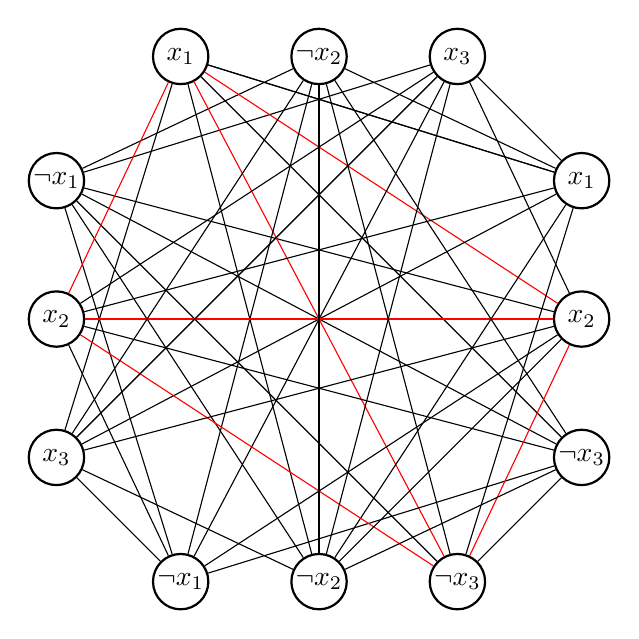
\begin{tikzpicture}
\node[state] (a1) {$\neg x_1$};
\node[state, below of=a1] (a2) {$x_2$};
\node[state, below of=a2] (a3) {$x_3$};

\node[state, above right =1.5cm of a1] (b1) {$x_1$};
\node[state, right of=b1] (b2) {$\neg x_2$};
\node[state, right of=b2] (b3) {$x_3$};

\node[state, below right =1.5cm of b3] (c1) {$x_1$};
\node[state, below of=c1] (c2) {$x_2$};
\node[state, below of=c2] (c3) {$\neg x_3$};

\node[state, below right =1.5cm of a3] (d1) {$\neg x_1$};
\node[state, right of=d1] (d2) {$\neg x_2$};
\node[state, right of=d2] (d3) {$\neg x_3$};

% \draw (a1) to (b1);
\draw (a1) to (b2);
\draw (a1) to (b3);
% \draw (a1) to (c1);
\draw (a1) to (c2);
\draw (a1) to (c3);
\draw (a1) to (d1);
\draw (a1) to (d2);
\draw (a1) to (d3);
\draw[red] (b1) to (a2);
\draw (b1) to (a3);
\draw (b1) to (c1);
\draw[red] (b1) to (c2);
\draw (b1) to (c3);
% \draw (b1) to (d1);
\draw (b1) to (d2);
\draw (b1)[red] to (d3);
\draw (c1) to (b1);
\draw (c1) to (b2);
\draw (c1) to (b3);
\draw (c1) to (a2);
\draw (c1) to (a3);
% \draw (c1) to (d1);
\draw (c1) to (d2);
\draw (c1) to (d3);
\draw (d1) to (b2);
\draw (d1) to (b3);
\draw (d1) to (c2);
\draw (d1) to (c3);
\draw (d1) to (a2);
\draw (d1) to (a3);

% \draw (a2) to (b2);
\draw (a2) to (b3);
\draw (a2)[red] to (c2);
\draw (a2) to (c3);
% \draw (a2) to (d2);
\draw (a2)[red] to (d3);
\draw (b2) to (a3);
% \draw (b2) to (c2);
\draw (b2) to (c3);
\draw (b2) to (d2);
\draw (b2) to (d3);
\draw (c2) to (b3);
\draw (c2) to (a3);
\draw (c2) to (d2);
\draw (c2)[red] to (d3);
\draw (d2) to (b3);
\draw (d2) to (c3);
\draw (d2) to (a3);

\draw (a3) to (b3);
% \draw (a3) to (c3);
% \draw (a3) to (d3);
\draw (b3) to (a3);
% \draw (b3) to (c3);
% \draw (b3) to (d3);
\draw (c3) to (d3);
\end{tikzpicture}
\caption{3-SAT to k-clique reduction of example (\ref{f1})}
\end{figure}

Notice that for each clause, there exits a node with neighbours from eavery other part. 
Therefore, there exists a 4-clique and by taking the literals from the nodes in the clique we have a valid solution to the 3-SAT problem.

\section{K-CLIQUE TO SAT}

We provide two methods to solve the problem of reducing k-clique to a SAT instance.
\subsection{Method 1}\label{s1}
In the first method we take $n$ variables, each representing one vertex in the graph $G = (V,E)$. We want to have a valid solution iff the variables that are \lstinline{true} correspond to a valid k-clique in the graph.
To achieve this we create the following constraints:

\begin{enumerate}
    \item For each unconnected pair of vertices, at least one vertex of the pair doesn't belong in a clique (If both do, it wouldn't be a clique since the two don't connect):
    \[ \forall (i, j) \notin E, \; \neq x_i \lor \neg x_j \]
    \item Then, check that at least k vertices are part of the clique. We do this by checking that for every combination of $n-(k-1)$ vertices there is at least one that is part of the clique:
    \[ \forall (i_1, i_2, \dots, i_{n-k+1}) \in (1, 2, \dots, n), \; \bigvee x_i \]
    This is the same as checking that there does there are no less than $k$ \lstinline{true} variables. 
    
    If there were less than $k$ \lstinline{true} variables in a solution, then there is a combination where taking $k-1$ variables removes all \lstinline{true} variables. 
    Therefore, if we check that for every possible combination of $k-1$ variables there is one or more \lstinline{true} in the others. Taking $k-1$ of $n$ elements and then looking at the rest is the same as taking $n-(k-1)$ elements.
    \end{enumerate}
This method has a complexity of $O\left(n^2+{{n}\choose{k-1}}\right)$ clauses.
\subsection{Method 2}    
Given a graph $G = (V,E)$ and a number $k$, we will have variables $x_{iv}$ for every 1$\leq$i$\leq$k and every v$\in$V. You should think of $x_{iv}$ as stating that v is the $ith$ vertex in the clique. We want to encode the following constraints:

\begin{enumerate}
\item 	For each i,j, the $ith$ vertex is connected to the $jth$ vertex only if there is an edge between the two: \[\forall v\in V, \forall(i,j)\in \{1,\dots,k\}, \; \neg x_{iv} \lor x_{ju_1} \lor \dots \lor x_{ju_m}\], s.t. $u_{1,\dots,m}$ are the neighbours of $v$.
\item 	For each $i\in(1,\dots,k)$, there is an $ith$ vertex in the clique: \[\forall i\in \{1,\dots,k\}, \; x_{i1} \lor x_{i2} \lor x_{i3} \lor \dots \lor x_{iv}\]
\item   For each $i\in(1,\dots,k)$, We need to check that there is at most one vertex in position $i$: \[\forall(x_{ia},x_{ib})\in x_i, \; \neg x_{ia} \lor \neg x_{ib}\]
\end{enumerate}

If we take all these clauses together, we get a CNF which states that "the $x_{iv}$ encode a k-clique in G". This CNF is satisfiable if and only if G contains a k-clique.
This method has a complexity of $O(k^2+kn^2)$ clauses.

\section{CODE}
In this section we will show the code for solving the problem using the first method seen in Section \ref{s1}.
The \textit{solve()} function will create clauses for pairs of vertices that are not connected to each other. It will do this in the following way:

\begin{itemize}
\item First we check that the size (which we have stored in the variable called "size") is equal to 0. If it is, we will return an error message since the network must contain at least one vertex (otherwise it is unsolvable and makes no sense).
\item If it is not, we continue.
\end{itemize}
We consider the edges as a lower triangular adjacency matrix, in which in the first row will appear the connections that vertex 0 has, in the second row those of vertex 1, and so on until the last vertex (being 0 not connected with another vertex and 1 connected with another vertex).\newline

For example, if we have 5 vertices and vertex 0 is connected to vertices 1 and 3, the first column of the matrix will be the following: 0 1 0 1 0 0

Therefore, we will go through the matrix row by row and column by column, i.e. element by element. 

For each element of the matrix:

\begin{itemize}
\item If it is 1, i.e. the vertices are connected to each other, we continue.
\item If it is 0, i.e. the vertices are not connected, we create a clause, since that row and that column (i.e. that pair of vertices) cannot be in the clique.
\end{itemize}

\leftskip=0.5in
Then we call the function \textit{recursiveClauses()}, this function computes the rest of the clauses to make sure that at least k variables are true.

Once we have this, we will join the clauses created for the unconnected vertices with the clauses for the connected vertices, which will form our solution.

We will pass these clauses created for a given size to the \textit{satSolve()} function. If it does not find a solution, no solution will be displayed, but if it does, it will be displayed. There may be more than one possible clique within a network for a given size k. This function will display one of the possible solutions at random.\newline

The code of the function is as follows:

\begin{lstlisting}
    Function solve() {
	let size = instanceVertexCount;
    	let clauses = []
        if (size == 0) throw("Graph must contain at least 1 vertex")
        for (row in instance) {
            for (col in instance[row]) {
                // For each possible combination of vertices
                if (!instance[row][col]) {
                    // If there is no edge create a clause
                    // "Either row or col are not in the clique"
                    clauses.push([-(parseInt(row)+1), -(parseInt(col)+1)])
                }
            }
        }
        let others = recursiveClauses(size - k + 1)
        clauses = clauses.concat(others)
        let solution = satSolve(size, clauses)
        if (!solution) return solution 
        return solution.filter(i => i>0).map(i => i-1)
    }

\end{lstlisting}

As we have already said, the function \textit{recursiveClauses()} computes the rest of the clauses to make sure that at least k variables are true. 
We will call this function recursively, creating a vector for each iteration in which we will add clauses for each vertex, until we reach the last vertex where we will stop the recursion.

The code of the function is as follows:

\begin{lstlisting}
    function recursiveClauses(stop, v = [], j = 0) {
    let out = []
        if (v.length == stop) return [v]
        for (let i = j; i < instanceVertexCount; i++) {
            next = [...v]
            next.push(i+1)
            out = out.concat(recursiveClauses(stop, next, i+1))
        }
        return out
    }

\end{lstlisting}

\section{GUI}
The program comes with a Graphical User Interface, where users are able to build, download and upload graphs and solve the k-clique problem for a desired value of $k$.

It is accessible from \url{https://abuafi.github.io/cliqueSAT/}.

It is also possible to add the \lstinline{debug} url parameter to see information for every problem instance solved and to run the tests in the next section. (\url{https://abuafi.github.io/cliqueSAT?debug=true})

\section{TEST CASES}
\begin{figure}[h]
    \centering
    \begin{subfigure}{0.49\linewidth}
        \scalebox{0.5}{\includegraphics{figures/Figure_insect_time.png}}
        \subcaption{Insect preset}
    \end{subfigure}
    \begin{subfigure}{0.49\linewidth}
        \scalebox{0.5}{\includegraphics{figures/Figure_icosagon_time.png}}
        \subcaption{Icosagon preset with full clique}
    \end{subfigure}
    \begin{subfigure}{0.49\linewidth}
        \scalebox{0.5}{\includegraphics{figures/Figure_icosagon_random_time.png}}
        \subcaption{Icosagon preset with random edges}
    \end{subfigure}
    \begin{subfigure}{0.49\linewidth}
        \scalebox{0.5}{\includegraphics{figures/Figure_fish_time.png}}
        \subcaption{Icosagon preset with random edges}
    \end{subfigure}
    \caption{Recorded times for the program to solve each preset at different values of $k$. (Times are given in milliseconds)}\label{g1}
\end{figure}
We have prepared a few tests to show the algorithm running on real graphs.
To gather the data for the test, run the function \lstinline{runTests()} in the browser console. 
In case any test fails (the program returns the wrong solution), an error will be thrown.

After a few minutes, you will be able to download the data which the Figures \ref{g1} and \ref{g2} show.

Figure \ref{g1} shows the time taken to solve each instance. 
We can see that the first method (here labeled with "solve") 
performs worse for low values of $k$ than the second method (here labeled with "solve\_alt").

Notice how method 2 begins losing the advantadge when $k$ surpasses the satisfiable threshold: In the "insect" preset the graph is only satisfiable for $k\leq 6$ and for the "fish" preset it is satisfiable for $k\leq 5$.

This is not due to the complexity of the number of clauses but rather the speed at which the SAT solver is able to find a solution.
\begin{figure}[h]
    \centering
    \begin{subfigure}{0.49\linewidth}
        \scalebox{0.5}{\includegraphics{figures/Figure_insect_clauses.png}}
        \subcaption{Insect preset}
    \end{subfigure}
    \begin{subfigure}{0.49\linewidth}
        \scalebox{0.5}{\includegraphics{figures/Figure_fish_clauses.png}}
        \subcaption{Icosagon preset with random edges}
    \end{subfigure}
    \caption{Number of clauses generated by each preset at different values of $k$.}\label{g2}
\end{figure}
\pagebreak
\section{MATERIALS}
The following resources are not made by us but are included with the program/GUI:
\begin{itemize}
    \item\href{https://www.comp.nus.edu.sg/~gregory/sat/sat.js}{sat.js}, a SAT solver for JavaScript. A slight modification was made in order to return a valid solution in case the problem is satisfiable.  
    \item\href{https://github.com/ubilabs/kd-tree-javascript}{k-d Tree JavaScript Library}, used for the front-end of the GUI.
    \end{itemize}
\section{BIBLIOGRAPHY}
\begin{itemize}
\item\href{https://en.wikipedia.org/wiki/Clique_problem}{Clique problem}    
\item\href{http://www.cs.ecu.edu/karl/6420/spr16/Notes/NPcomplete/3sat.html}{3 SAT}    
\item\href{https://www.geeksforgeeks.org/proof-that-clique-decision-problem-is-np-complete}{CLIQUE is NP-complete}    
\item\href{https://opendsa-server.cs.vt.edu/ODSA/Books/Everything/html/threeSAT_to_clique.html}{SAT to clique}    
\item\href{https://paperzz.com/doc/7301675/3sat-reduction-to-clique}{reduction to clique} 
\item\href{https://en.wikipedia.org/wiki/Boolean_satisfiability_problem}{Boolean satisfiability problem}
\item\href{https://www.cs.umd.edu/~gasarch/TOPICS/sat/SATtalk.pdf}{SAT}
\item\href{https://logic4free.informatik.uni-kiel.de/llocs/Conjunctive_normal_form_(propositional_logic)}{Conjunctive normal form}
\item\href{https://cs.stackexchange.com/questions/70531/reduction-3sat-and-clique}{reduction 3 sat to clique}
\item\href{https://dl.acm.org/doi/10.1145/800157.805047}{Cook's theorem}
\end{itemize}

\end{document}
